% !TeX spellcheck = en_US
%%
%% sample document for AAMAS'18 conference
%%
%% modified from sample-sigconf.tex
%%
%% see ACM instructions acmguide.pdf
%%
%% AAMAS-specific questions? n.yorke-smith@tudelft.nl
%%

\documentclass[sigconf]{aamas}  % do not change this line!

%% your usepackages here, for example:
\usepackage{booktabs}
\usepackage{graphicx}
\usepackage[rflt]{floatflt}
\usepackage{subcaption} 
\usepackage{frame, caption}
\usepackage{amsmath}
\usepackage{mathrsfs}
\usepackage{array}

\newcommand{\argmax}{\operatornamewithlimits{arg\,max}}

%% do not change the following lines
\setcopyright{ifaamas}  % do not change this line!
\acmDOI{doi}  % do not change this line!
\acmISBN{}  % do not change this line!
\acmConference[AAMAS'18]{Proc.\@ of the 17th International Conference on Autonomous Agents and Multiagent Systems (AAMAS 2018), M.~Dastani, G.~Sukthankar, E.~Andre, S.~Koenig (eds.)}{July 2018}{Stockholm, Sweden}  % do not change this line!
\acmYear{2018}  % do not change this line!
\copyrightyear{2018}  % do not change this line!
\acmPrice{}  % do not change this line!

%% the rest of your preamble here


%%%%%%%%%%%%%%%%%%%%%%%%%%%%%%%%%%%%%%%%%%%%%%%%%%%%%%%%%%%%%%%%%%%%%%%%%%%%%%%%%%%%%%%%%%%%%%%%%%%%%%%%%

%%%%%%%%%%%%%%%%%%%%%%%%%%%%%%%%%%%%%%%%%%%%%%%%%%%%%%%%%%%%%%%%%%%%%%%%%%%%%%%%%%%%%%%%%%%%%%%%%%%%%%%%%

\begin{document}
	
	\title{I've got the power's value! A computational model to evaluate the interlocutor's behaviors in collaborative negotiation}  % put your title here!

	\subtitle{Socially Interactive Agents Track}

	
	% AAMAS: submissions are anonymous for most tracks
%	\author{Paper \#32}  % put your paper number here!
	

	%
	\author{Lydia OuldOuali}
	\affiliation{%
	  \institution{LIMSI-CNRS}
	  \streetaddress{Universit\'e Paris-Sud}
	  \city{Orsay, France } 
	}
	\email{ouldouali@limsi.fr}
	
	\author{Nicolas Sabouret}
	\affiliation{%
		\institution{LIMSI-CNRS}
		\streetaddress{Universit\'e Paris-Sud}
		\city{Orsay, France } 
	}
	\email{nicolas.sabouret@limsi.fr}
	
	
	\author{Charles Rich}
	\affiliation{%
		\institution{Worcester Polytechnic Institute}
		\streetaddress{}
		\city{Worcester, Massachusetts, USA} 
	}
	\email{rich@wpi.edu}
	

	
	\begin{abstract}  % put your abstract here!
		We present in this paper a simulation-oriented theory of mind model for interpreting behaviors of power during a collaborative negotiation. This model relies on a model of negotiation that allows an agent to express behaviors of power through its strategy of negotiation. Based on the \emph{simulation theory}, we adapted the decision model of the agent to reason about its interlocutor's behavior. A preliminary evaluation in the context of agent-agent interaction shows that the system correctly predicts the interlocutor's power.
	\end{abstract}
	

	\keywords{Dominance; Reasoning about other; Theory of mind}  % put your semicolon-separated keywords here!
	
	\maketitle

	
	\section{Introduction}
	
	Negotiation is a common task in daily life. People negotiate not only in professional situations (\emph{e.g.} for a salary increase or a promotion) but also in more simple situations such as choosing the holiday's destination. In the last decade, a variety of conversational agents have been created that can negotiate with people \cite{pynadath2013you,gratch2016misrepresentation,klatt2011negotiations}.
	
	Research in social psychology demonstrated that the relation of dominance affects the way that the negotiation process is perceived \cite{van2006power}. Negotiators build different negotiation strategies depending on their relative dominance which directly influences the outcomes of the negotiation. More precisely, Tidens \cite{tiedens2003power} showed that dominance complementarity (\emph{i.e.} one negotiator exhibits dominant behaviors while the other one responds with submissive ones) leads the negotiators to reach mutually beneficial outcomes and increases their reciprocal likings.
	
	In this poster, we present an agent that simulates such a relation of dominance in collaborative negotiation, based on the computational model proposed by \cite{ouali2017computational}. We show how this model can be adapted to reason about the interlocutor's power, following a Theory of Mind approach to simulate the mental activity of the interlocutor. We show that the agent can make good predictions in the context of agent-agent interaction.
	
	\begin{figure*}
		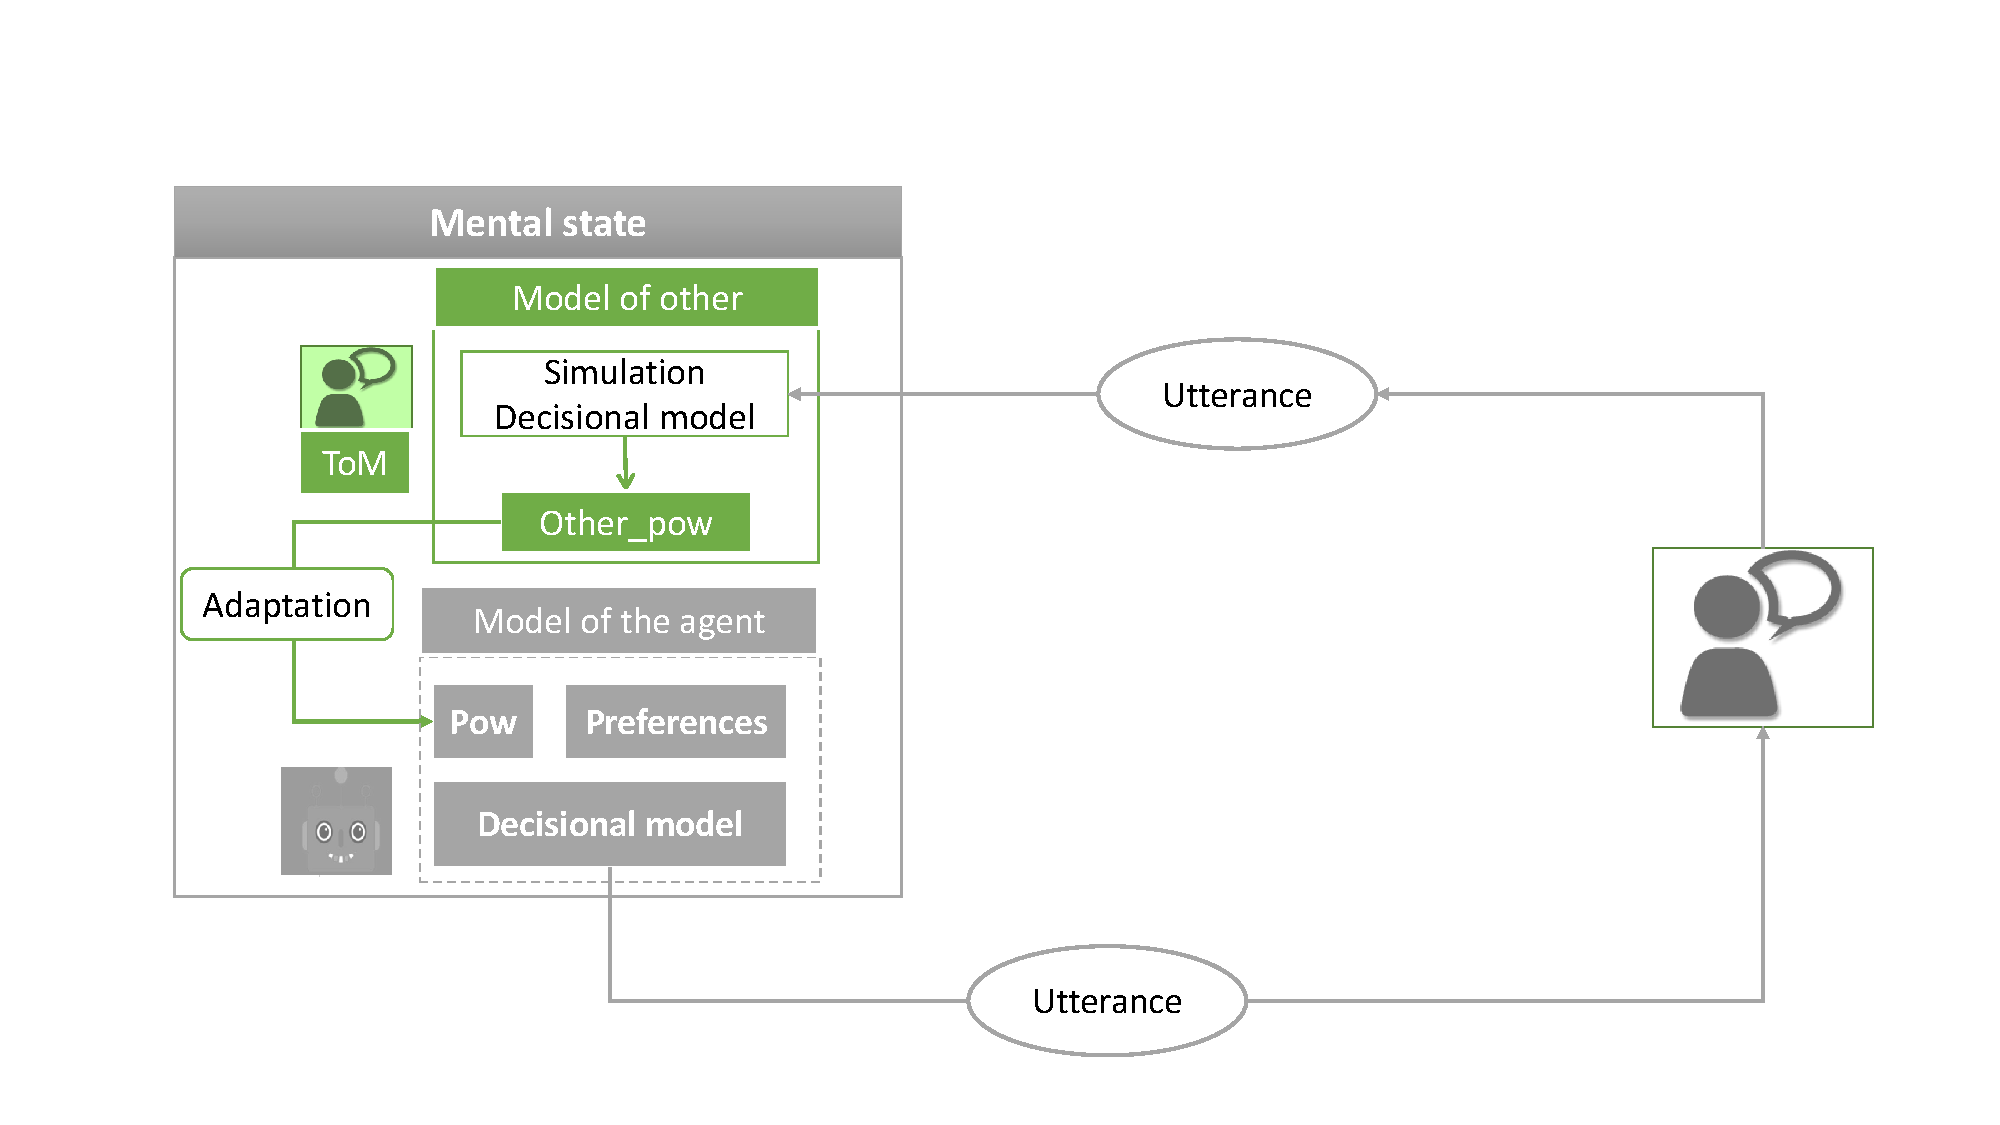
\includegraphics[width=0.7\linewidth]{figs/model_tom.pdf}
		\caption{Model of collaborative negotiation with a model of other} 
		\label{fig:schema-general}
	\end{figure*} 


	\section{Negotiator agent with ToM}
	Our negotiator agent can handle a negotiation to choose one option over several ones, characterized different criteria values. For example, the negotiation for a restaurant considers the criteria \textit{Cuisine, atmosphere, price and location}. The agent has a set of \textit{binary preferences} $\prec_i$ on each criterion $i$. It communicates with its interlocutor via abstract \emph{utterances} (\emph{i.e.} formal speech acts) to either share its preferences or make negotiations moves. An example of a dialogue is presented in Figure \ref{fig:ex-dia}. 
				
					\begin{figure}[b]
						 \begin{minipage}{.48\textwidth}
								\slshape
								%\begin{addmargin}[1em]{2em}% 1em left, 2em right
								\textbf{A:} "Let's go to a restaurant at Montparnasse."
								
								\hspace*{3mm}\textbf{B:} "Okay, let's go to a restaurant at Montparnasse."
								
								$\ldots$
								
								\textbf{A:} "Do you like expensive restaurants?"
								
								
								\hspace*{3mm}\textbf{B:} "I don't like expensive restaurants."
								
								\textbf{A: }"Do you like affordable restaurants?"
								
								\hspace*{3mm}\textbf{B:} "Let's go to the Maison blanche restaurant. 
								$\\$It's a modern, cheap French restaurant on the Montparnasse"
								
								\hspace*{3mm}\textbf{A:} "Okay, let's go to the Maison blanche restaurant."
								%	\end{addmargin}
							\end{minipage}
							
						
						\caption{\label{fig:ex-dia}Example of dialogue.}
					\end{figure}
		
		As presented on Figure \ref{fig:schema-general}, the decision model takes into account the agent's preferences in addition to a value of power $pow \in  [0,1]$. The negotiation strategy selects an \emph{utterance} that the agent communicates to its interlocutor. 
	
		Based on the \emph{simulation theory}, we use the agent's decisional model to reason about the interlocutor's behaviors during the negotiation: the agent infers its interlocutor's value of power based on the utterances it received during the negotiation. To this purpose, the agent makes assumptions about the interlocutor's preferences and power. The algorithm is as follows:
	
		\begin{enumerate}
			\item Build a set $H_{pow}$ of hypothesis about power: $h\in H_{pow}$ represents the hypothesis $pow=h$. In our work, we consider only 9 values: 
			
			$H_{pow}=\{0.1, 0.2, \ldots, 0.9\}$.
			\item For each hypothesis $h$, build the set of all possible preferences $Prec_h$: the elements $p\in Prec_h$ are partial orders on the criteria.
			\item After each utterance $u$, remove all elements in $Prec_h$ that are not compatible with $u$. Concretely, if the applicability condition of $u$ is not satisfied in $p\in Prec_h$, then $p$ must be removed from the candidate mental states.
			\item For each $h$, generate the corresponding utterance using $h$ as input for the decisional model.
			\item Compute a score $score(h)$ based on the size of remaining hypothesis $|Prec_h|$ that generate an output similar to the utterance, $Utterance_{other}$ stated by the interlocutor. 
			\item 	The hypothesis with the highest score is the most probable value for the interlocutor's power value.
			
			\begin{equation}
			pow_{other} = \operatorname*{arg\,max}_{h} (score(h))
			\end{equation}
			
		\end{enumerate}
		
		This model however requires to build an important number of hypotheses for the agent to consider at each turn. Indeed, given a topic with $n$ criteria, assuming that each criterion has $k$ values, the number of hypotheses on the preference set that the agent has to compute is in the order of  $\prod_{i=1}^n (k+1)!$. For a topic with 5 criteria, 4 values each, the number of hypotheses to consider is $24.10^9$!
		
		To overcome this limitation, we consider only a \textit{partial representation} of the interlocutor's preferences. This solution is supported  by research in cognitive psychology: Harbers \cite{harbers2009modeling} suggests that, in order to simulate another's mental processes, it is not necessary to categorize all the beliefs and desires attributed to that person as such. In other words, it is not necessary to have a complete model of the interlocutor.
		
		Instead of computing all the possible relation of preferences $\prec_i$, we only compute the set of satisfiable values (\emph{i.e.} the values that the interlocutor likes). The set of hypotheses to consider is drastically reduced but 1) we had to adapt the agent's decision model in the simulation Theory of Mind in order to handle uncertainty of preferences in the reasoning process and 2) the inferred power value might not be correct since it relies on a different model (with uncertainties). 
		
		We conducted an experimental study to assess the validity of the decisional model with partial preferences. We implemented two agents with this model. At each dialogue turn, each agent will try to predict the behavior of power expressed by its interlocutor. For each agent, we compared the agent's prediction with the effective value of power assigned to other agent. We further analyzed the speed of the prediction and the timeliness of the algorithm. 
		
		The results obtained confirmed the accuracy of our model to predict the behavior of power expressed by an interlocutor during a collaborative negotiation.  As a perspective, we intend to evaluate our model of decision to be able to \emph{simulate a complementary relation of dominance} between an artificial agent and a human user. The goal is to study the impact of a complementary relation on the outcome of the negotiation as well as the experience of the negotiation.

	
	%%%%%%%%%%%%%%%%%%%%%%%%%%%%%%%%%%%%%%%%%%%%%%%%%%%%%%%%%%%%%%%%%%%%%%%%%%%%%%%%%%%%%%%%%%%%%%%%%%%%%%%%%
	%% bibliography: see CFP for number of permitted pages
	
	\bibliographystyle{ACM-Reference-Format}  % do not change this line!
	\bibliography{bibliography}  % put name of your .bib file here
	
\end{document}